\documentclass[12pt,a4paper]{article}
\usepackage{amsmath}
\usepackage{amsfonts}
\usepackage{amssymb}
\usepackage{graphicx}
\usepackage{secdot}
\usepackage[left=2cm,right=2cm,top=2cm,bottom=2cm]{geometry}

\author{Shibayan Biswas, AE21B109\\ Department of Aerospace Engineering\\ IIT Madras}
\title{Assignment - 3}

\date{September 13, 2022}

\begin{document}

\maketitle
\section{Methods for establishing the roots of a function:}
In mathematics and computing, a root-finding algorithm is an algorithm for finding zeros, also called "roots", of continuous functions. A zero of a function f, from the real numbers to real numbers or from the complex numbers to the complex numbers, is a number x such that f(x) = 0. As, generally, the zeros of a function cannot be computed exactly nor expressed in closed form, root-finding algorithms provide approximations to zeros, expressed either as floating-point numbers or as small isolating intervals, or disks for complex roots (an interval or disk output being equivalent to an approximate output together with an error bound).
\subsection{Bisection Method:}
This method can be used with either a spreadsheet or a graphing calculator with spreadsheet capabilities. Basically, the bisection method squeezes in on the root from both sides by making use of the Intermediate Value Theorem. In essence, this theorem says that if f is a continuous function on [a, b] and the sign of f(a) is different from the sign of f(b), then there must be some point, c, in the interval such that f(c) = 0, and is thus a root of the function. The Bisection method uses this to squeeze in on the root in the following way. First, we can select an interval that contains the root we are looking for by looking at the graph. Second, we find the midpoint of the given interval, in this case (b - a)/2 = m, and then look at the function f evaluated at a, b, and m. Third we compare the signs of f(a), f(m) and f(b). f(m) will be one of three things. It will either have the sign of f(a), the sign of f(b), or it will be 0. If it is 0 (it usually isn't), then we stop because we have found the root we are looking for. Now, suppose that the sign of f(m) is equal to the sign of f(a). This implies that the root will be between m and b, and so we choose [m, b] as our new interval and repeat the process. Similarly, we replace b with m if the sign of f(m) equals the sign of f(b). Which ever the case we know that the root is in our new interval, and the endpoints of that interval have different signs. To "squeeze" in on the root we continue the process, until the desired accuracy is achieved.
\subsection{Newton's Method:}
There are in fact two ways of getting the similar results in a shorter number of iterations, Newton's Method and the Secant Method. Unfortunately, you need to know some calculus for Newton's method, and so it may not be appropriate for some high school students. Anyhow let me give you a brief description of how Newton's method works. First, we must make the assumption that the function, f, is differentiable on [a, b]. If it is, then f will have a definite slope at every point in [a, b]. Let (c, f(c)) be a point on the curve where c is in [a, b], so there is a tangent line at this point which is an approximation to the curve at that point. We can describe this line by
\begin{equation}
	\text{l}(x) = \text{f'}(c) \text{(x - c)} + \text{f}(c)
\end{equation}
Now we can take the zero of this line as an approximation to the zero of f. This zero can be represented by (c' represents the zero)
\begin{equation}
	\text{c'} = \text{c} -  \text{f}(c)/\text{f'}(c)
\end{equation}
We can now take the point c' as our starting point and repeat the process. In this way we get a sequence of values that come closer and closer to the root of f.
\subsection{Secant Method:}
The Newton-Raphson algorithm requires the evaluation of two functions (the function and its derivative) per each iteration. If they are complicated expressions it will take considerable amount of effort to do hand calculations or large amount of CPU time for machine calculations. Hence it is desirable to have a method that converges as fast as Newton's method yet involves only the evaluation of the function. Let $x_0$ and $x_1$ are two initial approximations for the root 's' of f(x) = 0 and f($x_0$) and f($x_1$) respectively, are their function values. If $x_2$ is the point of intersection of x-axis and the line-joining the points ($x_0$, f($x_0$)) and ($x_1$, f($x_1$)) then $x_2$ is closer to 's' than $x_0$ and $x_1$. The equation relating $x_0$, $x_1$ and $x_2$ is found by considering the slope 'm'. Secant method starts with two initial approximation $x_0$ and $x_1$ (they may not bracket the root) and then calculates the $x_2$ by the same formula as in Regula-Falsi method but proceeds to the next iteration without bothering about any root bracketing.
\section{Application of the above methods:}
As, generally, the zeros of a function cannot be computed exactly nor expressed in closed form, root-finding algorithms provide approximations to zeros, expressed either as floating-point numbers or as small isolating intervals, or disks for complex roots (an interval or disk output being equivalent to an approximate output together with an error bound).
\subsection{Finding the roots of the equations using two unique starting sets:}
We have been given three equations for which we have to find the roots using the Bisection Method, Newton's Method and Secant Method. the given equations are represented below:
\begin{equation}
	\text{$f_1$}(x) = \text{$x^3$} - \text{$3x^2$} - \text{$x$} + 9
\end{equation}
This is the first equation for which we have to use the above three methods that are Bisection Method, Newton's Method and Secant Method respectively. I have written the code for  three algorithms in the python file dedicated to this equation  and have found out the roots using two unique sets of values as prescribed in the question. I have attached the dedicated python file for this equation in the zip file that I will be submitting. Here I have also plotted the values of $\text{$f_1$}(x)$ against the number of iterations for both the starting sets for each of the methods that is shown below:
\clearpage
\begin{figure}[!ht]
	\begin{center}
		\framebox{
			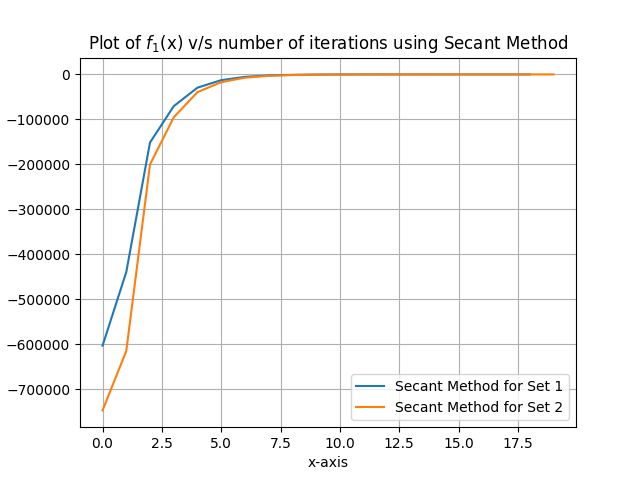
\includegraphics[scale=0.85]{Figure_1.png}
		}
	\end{center}
	\caption{Plot of $f_1$(x) v/s number of iterations using Secant Method}
\end{figure}
\begin{figure}[!ht]
	\begin{center}
		\framebox{
			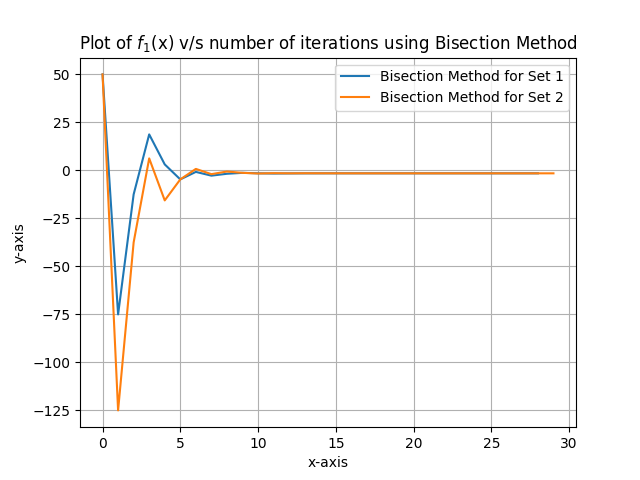
\includegraphics[scale=0.85]{Figure_2.png}
		}
	\end{center}
	\caption{Plot of $f_1$(x) v/s number of iterations using Bisection Method}
\end{figure}
\clearpage
\begin{figure}[!ht]
	\begin{center}
		\framebox{
			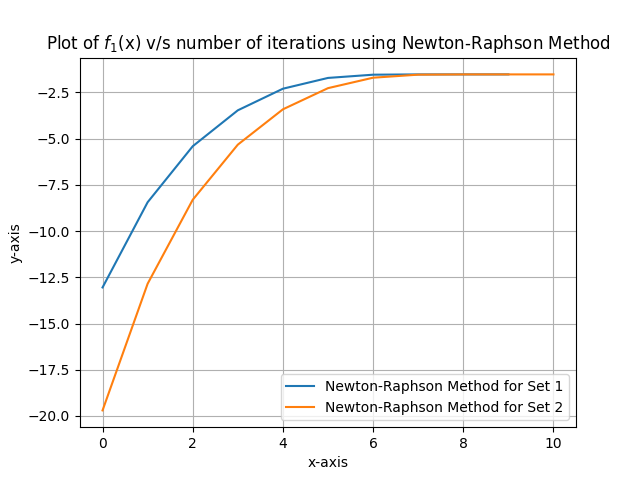
\includegraphics[scale=0.85]{Figure_3.png}
		}
	\end{center}
	\caption{Plot of $f_1$(x) v/s number of iterations using Newton-Raphson Method}
\end{figure}
\begin{equation}
	\text{$f_1$}(x) = \text{$e^x f_1(x)$}
\end{equation}
\\This is the second equation for which we have to use the above three methods that are Bisection Method, Newton's Method and Secant Method respectively. I have written the code for  three algorithms in the python file dedicated to this equation  and have found out the roots using two unique sets of values as prescribed in the question. I have attached the dedicated python file for this equation in the zip file that I will be submitting. Here I have also plotted the values of $\text{$f_2$}(x)$ against the number of iterations for both the starting sets for each of the methods that is shown below:
\clearpage
\begin{figure}[!ht]
	\begin{center}
		\framebox{
			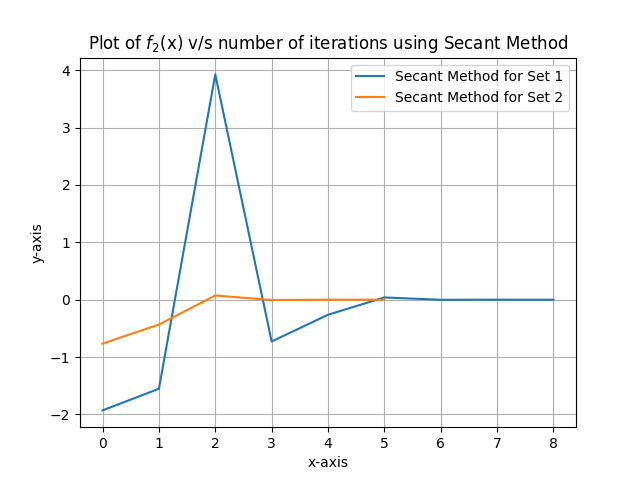
\includegraphics[scale=0.85]{Figure_4.png}
		}
	\end{center}
	\caption{Plot of $f_2$(x) v/s number of iterations using Secant Method}
\end{figure}
\begin{figure}[!ht]
	\begin{center}
		\framebox{
			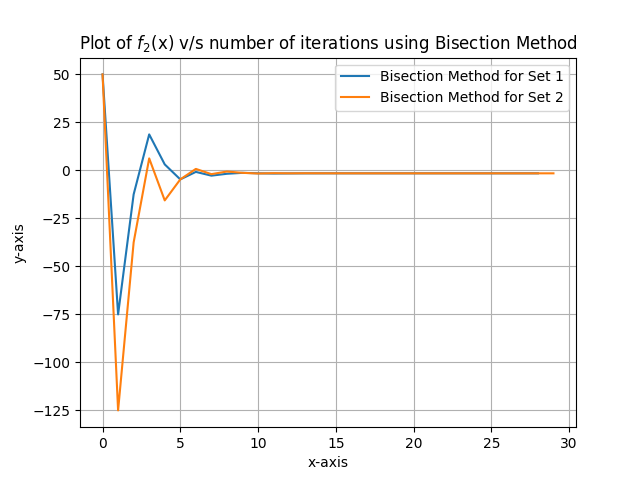
\includegraphics[scale=0.85]{Figure_5.png}
		}
	\end{center}
	\caption{Plot of $f_2$(x) v/s number of iterations using Bisection Method}
\end{figure}
\clearpage
\begin{figure}[!ht]
	\begin{center}
		\framebox{
			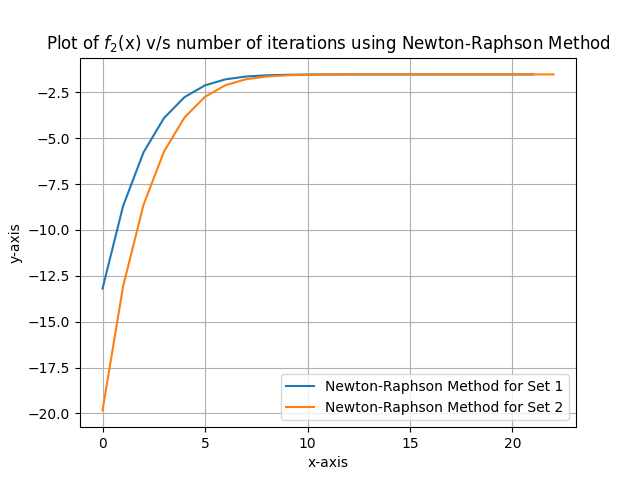
\includegraphics[scale=0.85]{Figure_6.png}
		}
	\end{center}
	\caption{Plot of $f_2$(x) v/s number of iterations using Newton-Raphson Method}
\end{figure}
\begin{equation}
	\text{$f_1$}(x) = \text{$x^3$} - \text{$2x$} + 2
\end{equation}
\\This is the third equation for which we have to use the above three methods that are Bisection Method, Newton's Method and Secant Method respectively. I have written the code for  three algorithms in the python file dedicated to this equation  and have found out the roots using two unique sets of values as prescribed in the question. I have attached the dedicated python file for this equation in the zip file that I will be submitting. In this case the nature of the plots for Bisection Method, Newton's Method and Secant Method will be more or less same as that of the first equation as this is also an equation of power three (same the first equation).
\subsection{Finding the roots of the equations for a given initial guess:}
In this case we have taken two sets of data as input from the user, one for the first equation (refer to equation 3) and the other for the second equation (refer to equation 4) and with reference to this data I have plotted the values of $\text{$f_2$}(x)$ against the number of iterations for each of equation 1 and equation 2. The sets of data taken from the user and the resultant plots are shown below:
\clearpage
\begin{figure}[!ht]
	\begin{center}
		\framebox{
			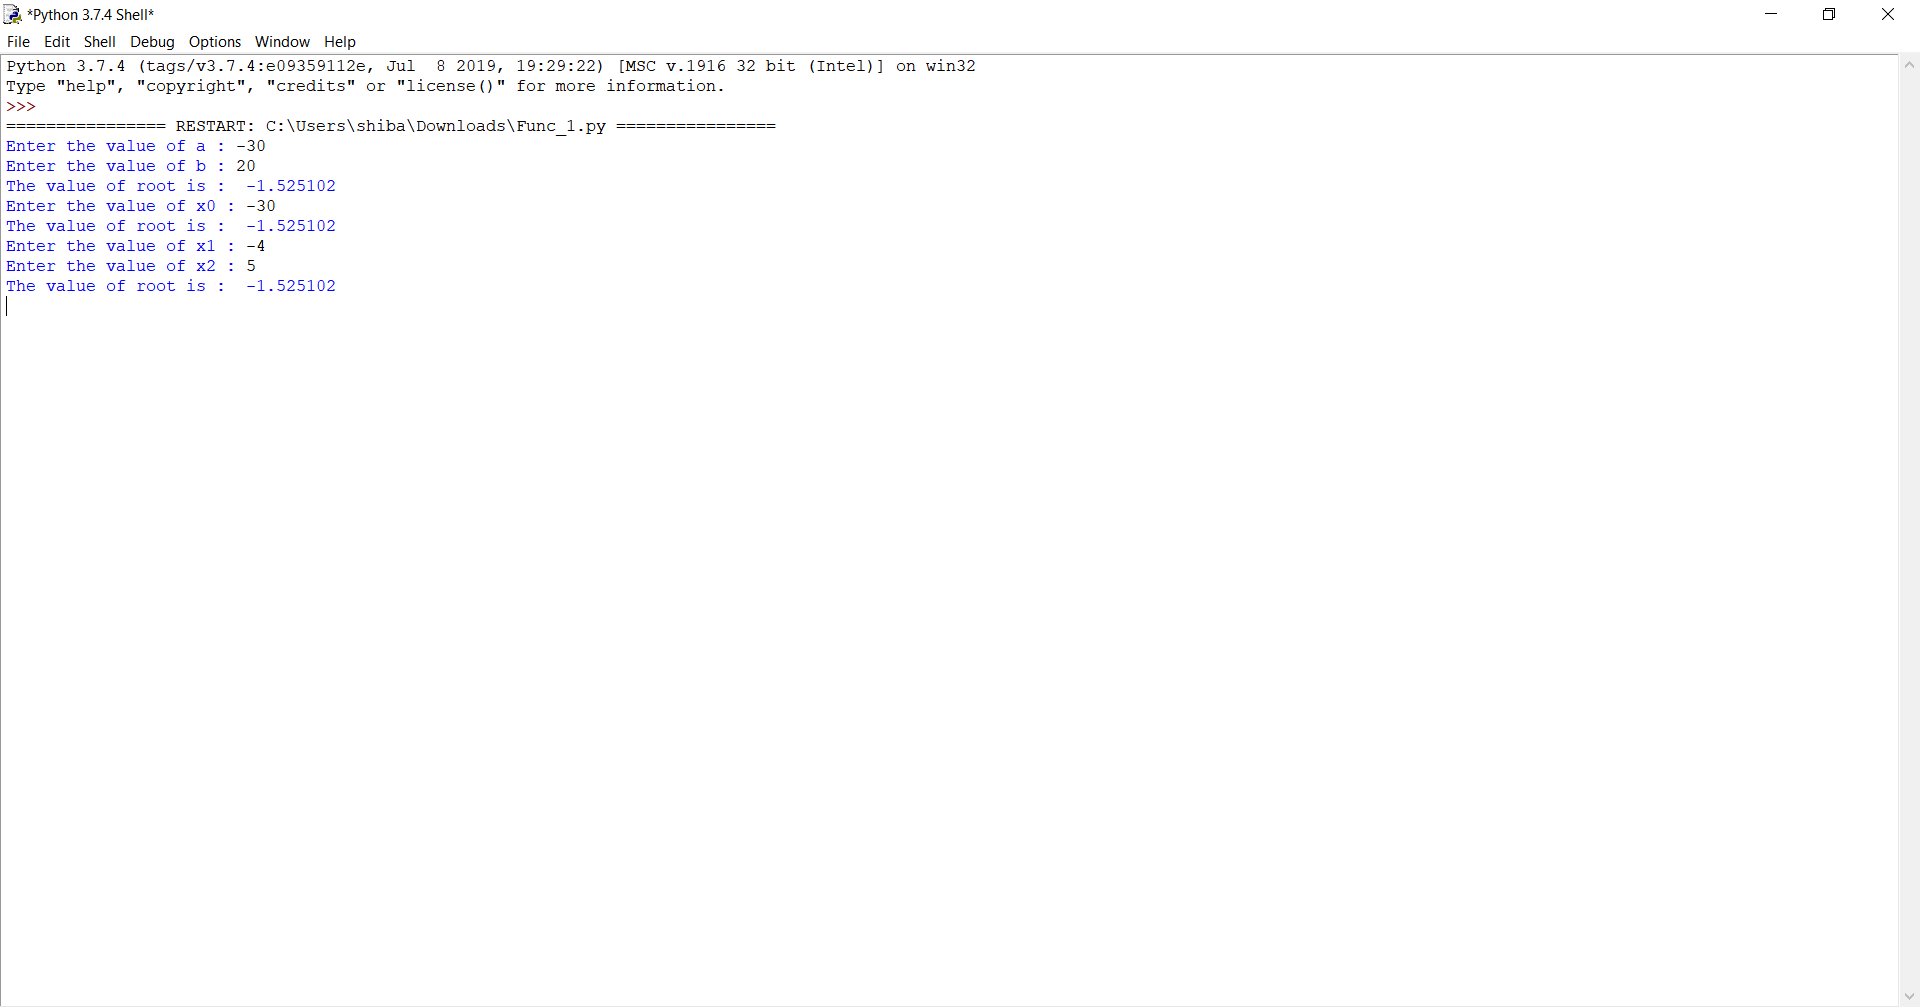
\includegraphics[scale=0.34]{User_Input_1.png}
		}
	\end{center}
	\caption{User input data for the different parameters to be used in finding the roots of $f_1(x)$}
\end{figure}
\begin{figure}[!ht]
	\begin{center}
		\framebox{
			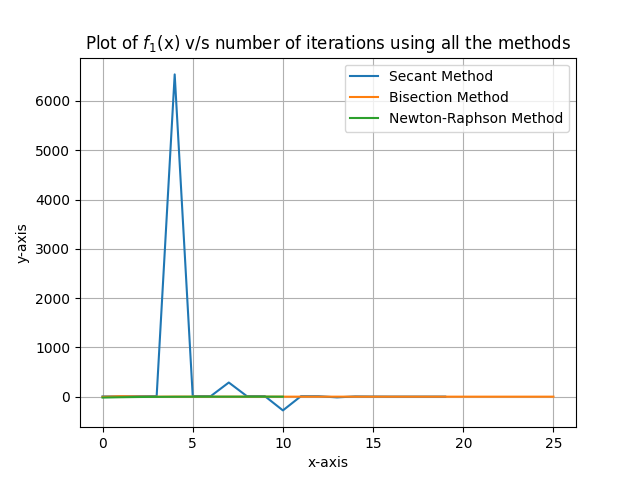
\includegraphics[scale=0.9]{Figure_7.png}
		}
	\end{center}
	\caption{Plot of $f_1$(x) v/s number of iterations using all the methods}
\end{figure}
\clearpage
\begin{figure}[!ht]
	\begin{center}
		\framebox{
			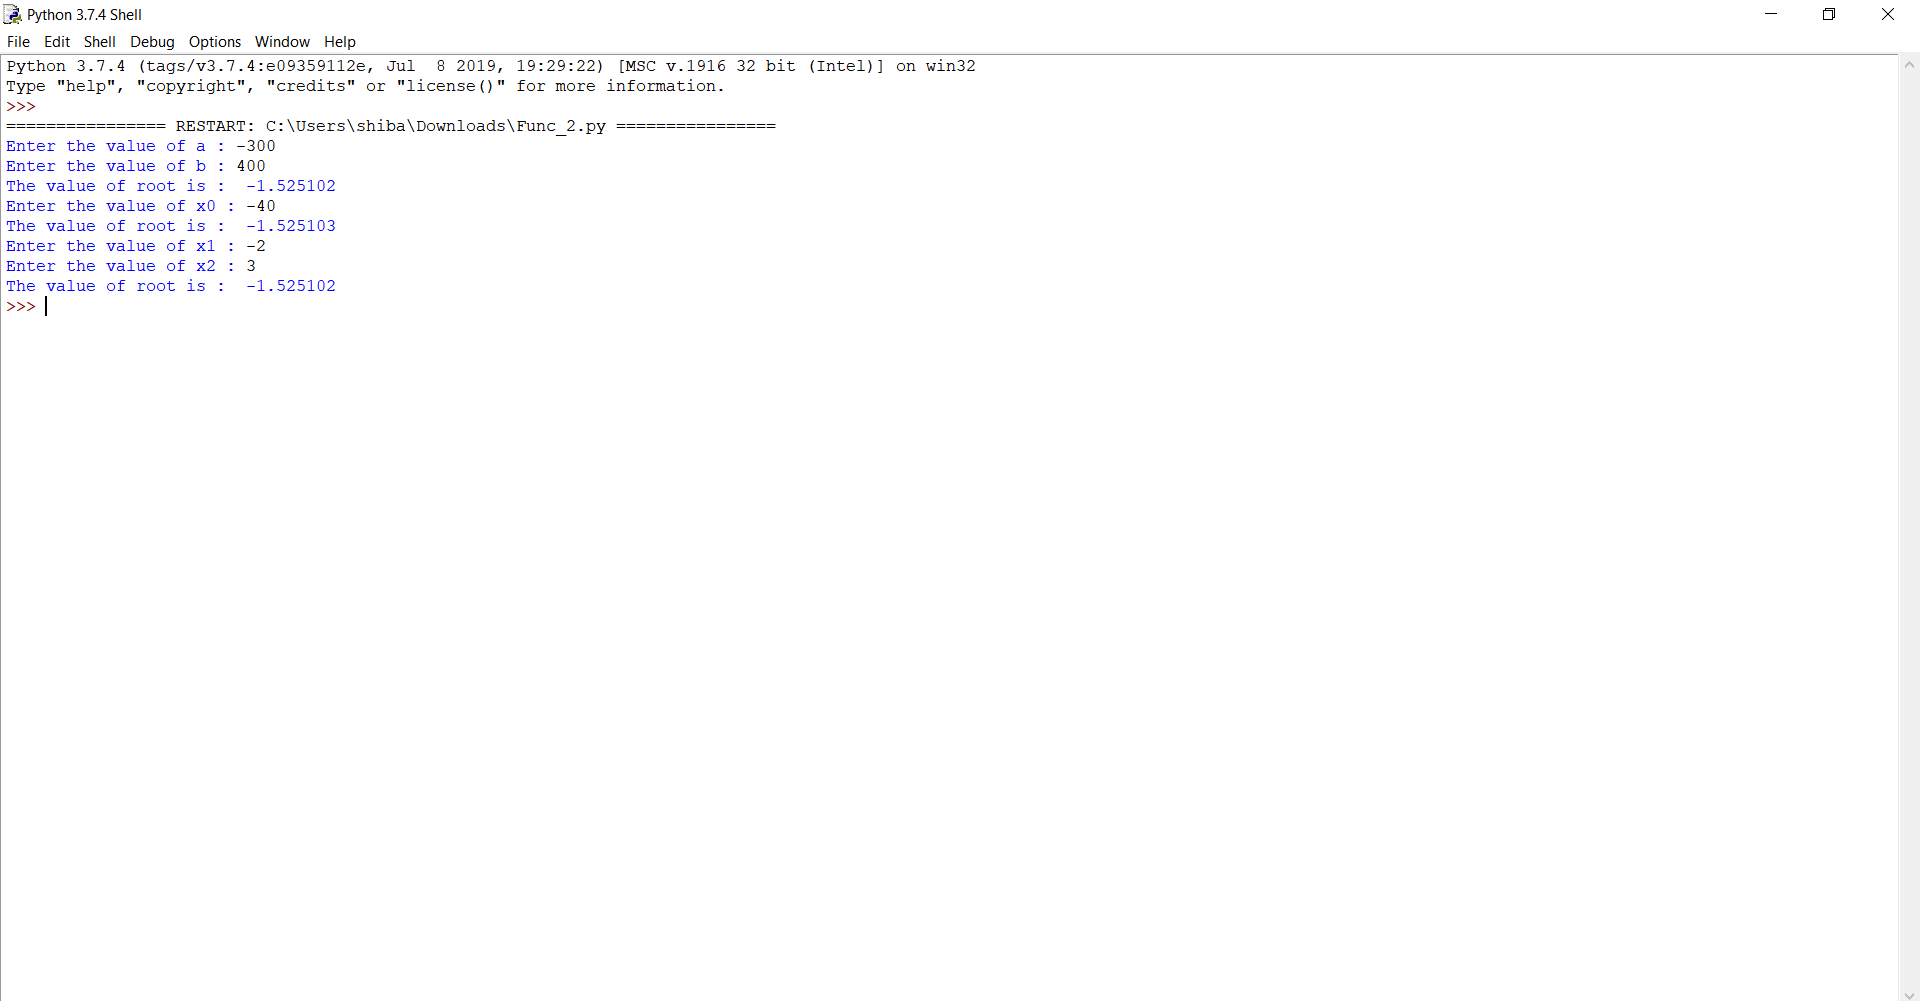
\includegraphics[scale=0.34]{User_Input_2.png}
		}
	\end{center}
	\caption{User input data for the different parameters to be used in finding the roots of $f_2(x)$}
\end{figure}
\begin{figure}[!ht]
	\begin{center}
		\framebox{
			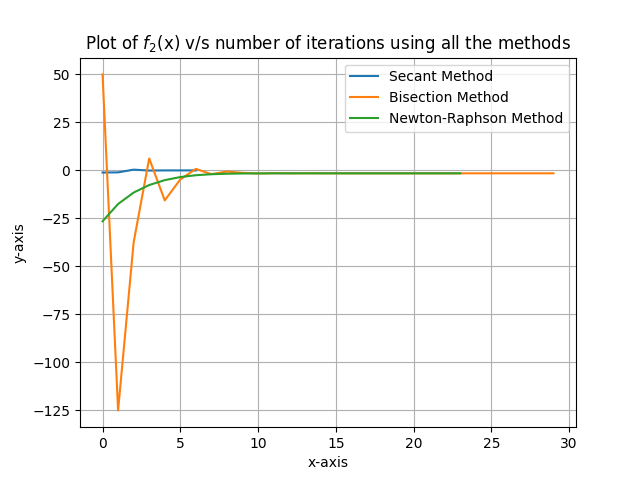
\includegraphics[scale=0.9]{Figure_8.png}
		}
	\end{center}
	\caption{Plot of $f_2$(x) v/s number of iterations using all the methods}
\end{figure}
\subsection{Representing the plots of $f_1$(x) and $f_2$(x) against wall-clock time:}
In this section I have represented the plots of $f_1$(x) and $f_2$(x) against wall-clock time for all of the three methods ie. Bisection Method, Newton's Method and Secant Method. It has been noticed that Newton's Method is the least time consuming algorithm followed by the Secant Method which is followed by the Bisection Method. The plots I have performed are shown below:
\begin{figure}[!ht]
	\begin{center}
		\framebox{
			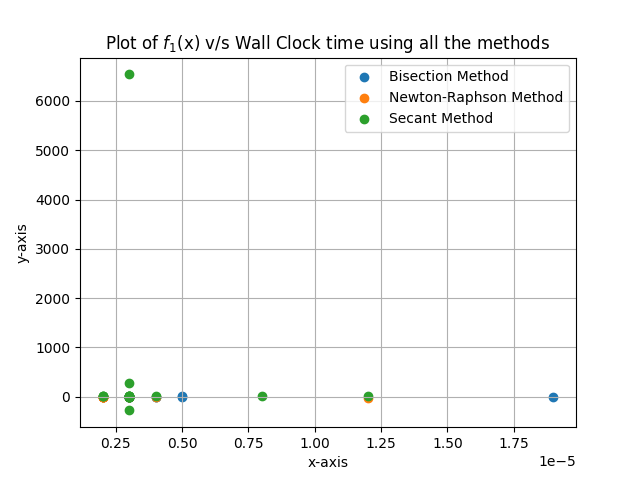
\includegraphics[scale=0.75]{Figure_9.png}
		}
	\end{center}
	\caption{Plot of $f_2$(x) v/s wall-clock time using all the methods}
\end{figure}
\begin{figure}[!ht]
	\begin{center}
		\framebox{
			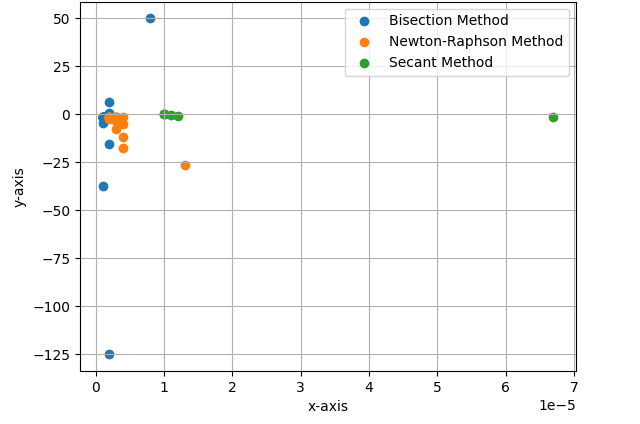
\includegraphics[scale=0.7]{Figure_10.png}
		}
	\end{center}
	\caption{Plot of $f_2$(x) v/s wall-clock time using all the methods}
\end{figure}
\section{Performing Newton's Method for $f_3$(x) with the starting guess as x = 0:}
At x = 0 the given equation $f_3$(x) has an inflection point. So at x = 0 the root of the tangent passing through it will be x = 1 and for the tangent passing through x = 1 the root of the tangent will be x = 0. Thus the point again comes to zero. So our loop will get trapped and these two values will never converge to give the root of the equation thus the program will keep running without producing any output. This scenario is represented by the image below:
\begin{figure}[!ht]
	\begin{center}
		\framebox{
			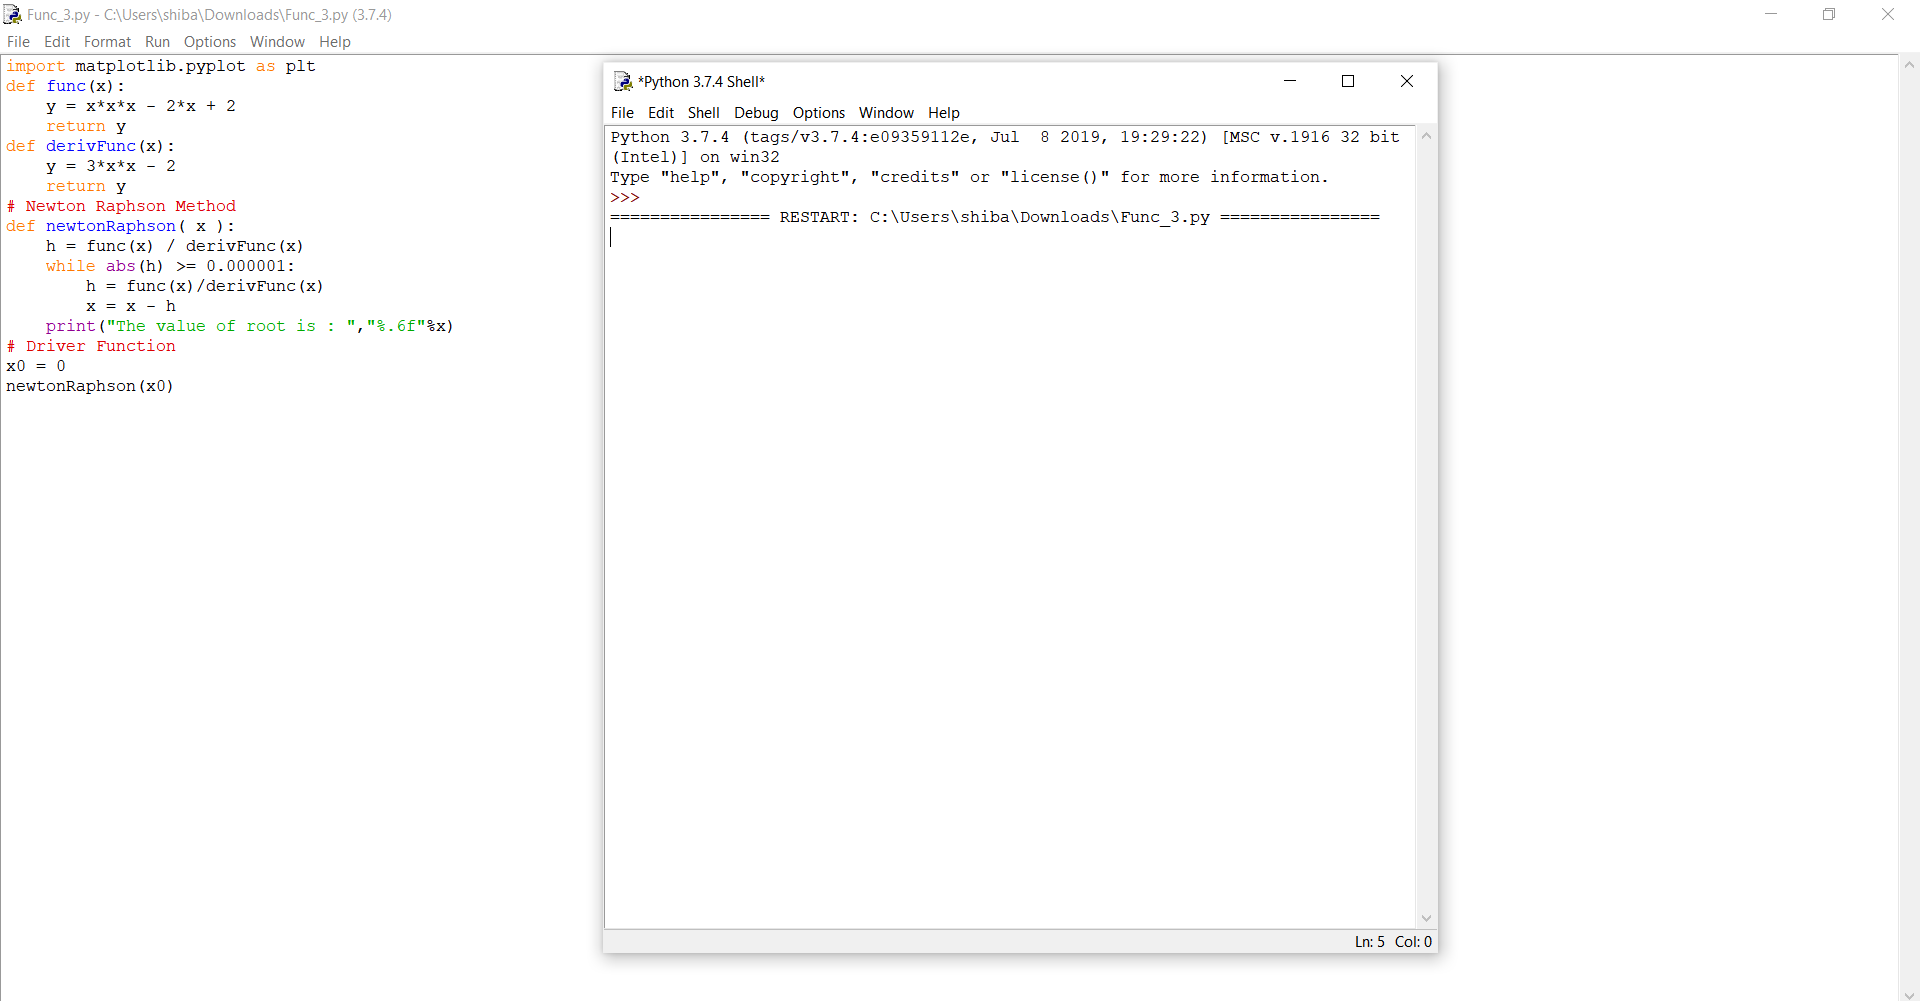
\includegraphics[scale=0.34]{Figure_11.png}
		}
	\end{center}
	\caption{Performing Newton's Method for $f_3$(x) with the starting guess as x = 0}
\end{figure}
\end{document}
